\subsection{Grafički prikaz frekvencijske funkcije odziva}
Zbog toga što frekvencijska funkcija pomaka definira uvećanje amplitude statičkog
pomaka (dinamički koeficijent pomaka) i fazno zaostajanje odziva za pobudom od posebnog 
su nam interesa kut i intenzitet frekvencijske funkcije odziva (polarni zapis).
\par

Za konstantan $\omega_n$ vrijednosti funkcija definiranih jednadžbama 
\eqref{eq:magnitudniSpektar} i \eqref{eq:fazniSpektar} biti će za omjer
$\omega/\omega_n$, stoga taj omjer možemo postaviti i kao argument navedenih
funkcija. 
\begin{equation}\label{eq:magnitudniSpektarZaOmjer}
    R_d = \left|H\left(\frac{\omega}{\omega_n}\right)\right|=
        \frac{1}{\sqrt{((1-(\omega/\omega_n)^2)^2+(2\zeta(\omega/\omega_n))^2}}
\end{equation}

\begin{equation}\label{eq:fazniSpektarZaOmjer}
    \phi\left(\frac{\omega}{\omega_n}\right)=
        \arctan\left(\frac{2\zeta(\omega/\omega_n)}{1-(\omega/\omega_n)}\right)
\end{equation}

\begin{figure}[H]
    \begin{subfigure}{1\textwidth}
        \input{./grafovi/sdf/rd-priguseno}
    \end{subfigure}
    \vfill
    \begin{subfigure}{1\textwidth}
        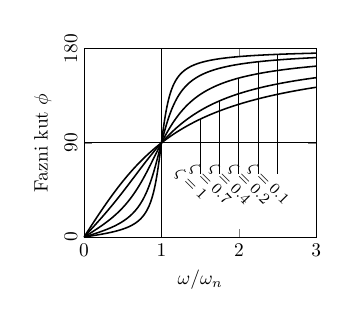
\begin{tikzpicture}[scale=0.7]
	\begin{axis} [
		height=5cm,
		ylabel = Fazni kut $\phi$, 
		xlabel = $\omega/\omega_n$,
		xmin = 0,
		xmax = 3,
		ymin = 0,
		ymax = 180,
		xtick = {0,1,2,3}, 
		ytick = {0,90,180}, yticklabel style={rotate=90},
	]

            \foreach \i in {1, 0.7, 0.4, 0.2, 0.1}
            {
                \addplot [
                    domain=0:1,
                    samples=200,
                    color=black,
                    thick
                ]{atan((2*x*\i)/(1-x^2))};
            }

            \foreach \i in {1, 0.7, 0.4, 0.2, 0.1}
            {
                \addplot [
                    domain=1.001:3,
                    samples=200,
                    color=black,
                    thick
                ]{180+atan((2*x*\i)/(1-x^2))};
            }
            \draw[thin](1.5,{180+atan((2*1.5*1)/(1-1.5^2))}) -- (1.5, 60)
                node[pos=1,rotate=-45,below] {\footnotesize{$\zeta=1$}};
            \draw[thin](1.75,{180+atan((2*1.75*0.7)/(1-1.75^2))}) -- (1.75, 60)
                node[pos=1,rotate=-45,below] {\footnotesize{$\zeta=0.7$}};
            \draw[thin](2,{180+atan((2*2*0.4)/(1-2^2))}) -- (2, 60)
                node[pos=1,rotate=-45,below] {\footnotesize{$\zeta=0.4$}};
            \draw[thin](2.25,{180+atan((2*2.25*0.2)/(1-2.25^2))}) -- (2.25, 60)
                node[pos=1,rotate=-45,below] {\footnotesize{$\zeta=0.2$}};
            \draw[thin](2.5,{180+atan((2*2.5*0.1)/(1-2.5^2))}) -- (2.5, 60)
                node[pos=1,rotate=-45,below] {\footnotesize{$\zeta=0.1$}};



        \draw[thin](1,0)--(1,180);
        \draw[thin](0,90) -- (3,90);
        \end{axis}
\end{tikzpicture}

    \end{subfigure}
    \caption{Dinamički koeficijent i fazni kut za prigušeni sustav pri harmonijskoj
    pobudi}
    \label{fig:frf-priguseno}
\end{figure}

Intenzitet frekvencijske funkcije odziva prikazuje funkcijsku ovisnost
dinamičkog koeficijenta $R_d$ o omjeru frekvencije pobude i prirodne frekvencije za
određeno prigušenje. Analogno tome fazni kut frekvencijske funkcije odziva
prikazuje kašnjenje u fazi za pobudom u ovisnosti o omjeru frekvencija 
$\omega/\omega_n$ za određeni faktor relativnog prigušenja.
\par

Za neprigušeno titranje, funkcije faznoga kuta i dinamičkog koeficijenta pomaka prikazane 
su u nastavku.
\begin{equation}\label{eq:fazniSpektarNepriguseno}
    \phi\left(\frac{\omega}{\omega_n}\right)=
        \arctan\left(\frac{0}{1-(\omega/\omega_n)}\right)
\end{equation}
\begin{equation}\label{eq:magnitudniSpektarNepriguseno}
    R_d=\left|H\left(\frac{\omega}{\omega_n}\right)\right|=
        \frac{1}{\sqrt{((1-(\omega/\omega_n)^2)^2+(2\cdot 0(\omega/\omega_n))^2}} =
        \frac{1}{|1-(\omega/\omega_n)^2|}
\end{equation}

Iz formule \eqref{eq:fazniSpektarNepriguseno} očito je da za neprigušeno titranje
postoje tri vrijednosti faznog kuta koje ovise o izrazu u nazivniku. Vrijednosti
faznog kuta prikazane su u nastavku:
\[
    \phi = \begin{dcases*}
            0\degree   & za $1-(\omega/\omega_n)^2 > 0$\\ % & $\omega < \omega_n$\\
            90\degree  & za $1-(\omega/\omega_n)^2 = 0$\\ % & $\omega = \omega_n$\\
            180\degree & za $1-(\omega/\omega_n)^2 < 0$\\ % & $\omega > \omega_n$\\
        \end{dcases*}
\]

\begin{figure}[H]
    \begin{subfigure}{1\textwidth}
        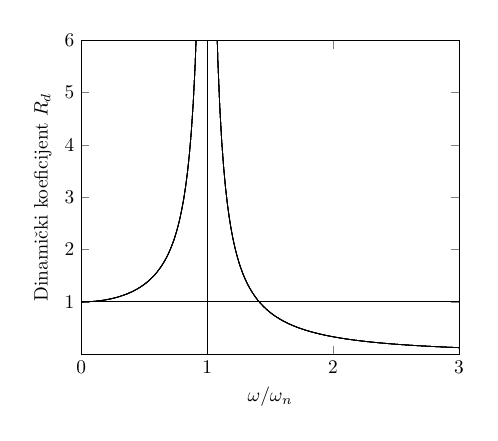
\begin{tikzpicture}[scale=0.7]
    \begin{axis} [
        ylabel = Dinamički koeficijent $R_d$,
        xlabel = $\omega/\omega_n$,
        xmin = 0, xmax = 3,
        ymin = 0, ymax = 6,
        xtick = {0, 1, 2, 3},
        ytick = {1, 2, 3, 4, 5, 6},
     ]

        \draw[thin] (1,0) -- (1,6);
        \draw[thin] (0,1) -- (3,1);
    \foreach \i in {1, 0.7, 0.4, 0.2, 0.1}
        {
            \addplot [
                domain=0:3,
                samples=200,
                color=black,
                thin,
            ]{1/abs(1-x^2)};
        }
    \end{axis}
\end{tikzpicture}

    \end{subfigure}
    \vfill
    \begin{subfigure}{1\textwidth}
        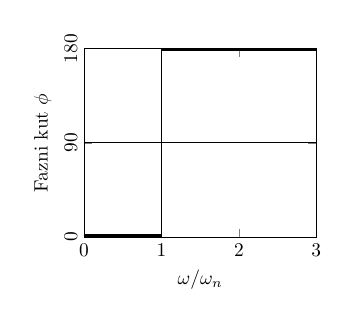
\begin{tikzpicture}[scale=0.7]
	\begin{axis} [
		height=5cm,
		ylabel = Fazni kut $\phi$, 
		xlabel = $\omega/\omega_n$,
		xmin = 0, xmax = 3,
		ymin = 0, ymax = 180,
		xtick = {0,1,2,3}, 
		ytick = {0,90,180}, yticklabel style={rotate=90},
	]
            \draw[thin] (0,90) -- (3,90);
            \draw[thin] (1,0)  -- (1,180);

        \addplot [
            domain=0:1,
            samples=200,
            color=black,
            line width=1mm,
        ]{atan((2*x*0)/(1-x^2))};
        \addplot [
                    domain=1.001:3,
                    samples=200,
                    color=black,
                    line width=1mm, 
       ]{180+atan((2*x*0)/(1-x^2))};
        \end{axis} 
\end{tikzpicture}

    \end{subfigure}
    \caption{Dinamički koeficijent i fazni pomak za neprigušeni sustav pri
    harmonijskoj pobudi}
    \label{fig:frf-nepriguseno}
\end{figure}
\newpage

Analizirajući krivulje sa \eqref{fig:frf-priguseno} i \eqref{fig:frf-nepriguseno} 
navedene grafove možemo podijeliti na tri područja (~\cite{chopra2011}):
\begin{enumerate}
    \item Područje kontrolirano krustošću - za slučaj spore promjene opterećenja
        ($\omega/\omega_n<<1$ - lijevo na grafu) utjecaj prigušenja je neznatan
        (krivulje za različita prigušenja su jako bliske) a dinamički utjecaj je mali, 
        tj. $R_d \approx 1$ što znači da je amplituda prisilnog odziva približno jednaka
        amplitudi statičkog pomaka, pa amplitudu prisilnog odziva možemo
        aproksimirati slijedećom jednadžbom:
        \begin{equation}\label{eq:frf_prvi_sektor}
            u_0\simeq(u_{st})_0=\frac{p_0}{k}
        \end{equation}
        Fazni kut je približno $0\degree$ pa su pobuda i odziv u fazi.

    \item Područje kontrolirano prigušenjem - Za slučaj $\omega/\omega_n\simeq 1$,
        izražen razmak između krivulja nalaže najeveći utjecaj prigušenja na
        vrijednost dinamičkog faktora, a samim time i na ukupnu amplitudu prisilnog
        odziva. Dinamički faktor $R_d$, u navedenom intervalu, postiže najveće
        vrijednosti a u slučaju $\zeta=0$ $R_d$ je neograničen (teži u beskonačno). 
        Dominantni član izraza \eqref{eq:magnitudniSpektarZaOmjer} je
        $2\zeta(\frac{\omega}{\omega_n})$, a aproksimacija amplitude prisilnog
        odziva glasi: 
        \begin{equation}\label{eq:frf_rezonanca}
            u_0=\frac{(u_{st})_0}{2\zeta}=\frac{p_0}{c\omega_n}
        \end{equation}

        Fazni kut za sva prigušenja iznosi 90\degree. 

    \item Područje kontrolirano masom - Za slučaj brze promjene opterećenja
        $\omega/\omega_n>>1$ utjecaj prigušenja je zanemariv jer su krivulje vrlo
        bliske. Dinamički faktor $R_d$ teži u nulu, što znači da je ukupna amplituda
        prisilnog odziva manja od amplitude statičkog pomaka. Dominantni član jednadžbe 
        \eqref{eq:magnitudniSpektar} jest $(\omega/\omega_n)^4$ što znači
        da jednadžbu pod \eqref{eq:magnitudniSpektarZaOmjer} možemo aproksimirati na 
        slijedeći način:
        \[
            H(\omega/\omega_n)\simeq \frac{\omega_n^2}{\omega^2}
        \]

        Prema tome, amplituda prisilnog odziva glasi:
        \begin{equation}\label{eq:frf_treci_sektor}
            u_0=(u_{st})_0\left(\frac{\omega_n}{\omega}\right)^2=\frac{p_0}{m\omega^2}
        \end{equation}
        
        U ovom slučaju ($\omega/\omega_n >> 1$), fazni kut je približno 180\degree,
        što znači da su pobuda i odziv izvan faze
\end{enumerate}



